\subsection{JPEG}
JPEG představuje jeden z nejpoužívanějších obrazových formátů (fotografie), jedná se o \textbf{ztrátový} formát obrázků. \textbf{Komprese JPEG} pracuje v několika krocích, principem je \textbf{redukce vysokofrekvenčních dat} v obrázků při zachování co nejvíce informací o nízkofrekvenčních datech. To je založeno na tom, že lidské oko se zaměřuje spíše na nízké frekvence (malou změnu jasu na ploše) a vysoké frekvence vnímá hůře (hrany). Můžeme si je tedy dovolit redukovat bez znatelné ztráty kvality obrazu. Zároveň se využívá \textbf{podvzorkování barev} $\rightarrow$ znovu z toho důvodu, že lidské oko vnímá více jas než barvy.

\begin{figure}[H]
	\centering
	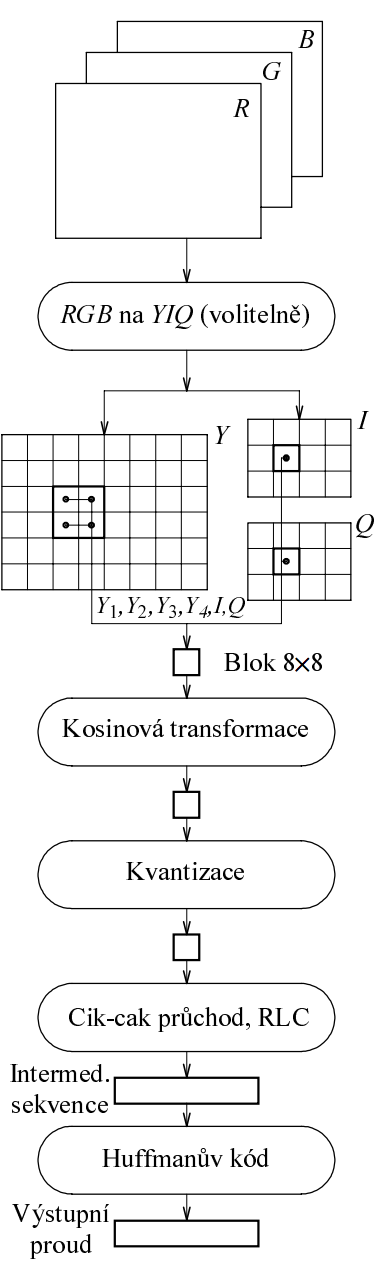
\includegraphics[width=0.3\textwidth]{assets/7_jpeg}
\end{figure}

\subsubsection{Komprese JPEG}
\begin{enumerate}
	\item \textbf{Převod RGB na YCbCr} -- vstupní obraz se převede na YCbCr, což jej rozdělí na \textbf{jasovou složku} (Y) a \textbf{chrominanční} složky (barvonosné Cb a Cr). To nám umožňuje následnou redukci barvonosné složky v jednom ze 3 módů: 4:4:4 (nepodvzorkovává se), 4:2:2 (horizontálně na polovinu, pro 2 jasové 1 barva), 4:2:0 (horizontálně i vertikálně na polovinu, pro 4 jasové 1 barva).
	\item \textbf{Provedení DCT} -- obraz se následně rozdělí na bloky o velikosti $8 \times 8$. Pro každý blok se provede 2D DCT (diskrétní kosinova transformace), ta narozdíl od DFT produkuje pouze reálné komponenty. Výsledek DCT nám vrátí počet jednotlivých frekvencí, které se v obraze nachází, přičemž \textbf{nízké frekvence} se koncentrují vlevo nahoře a \textbf{vysoké frekvence} vpravo dole (viz obrázek).
	\begin{figure}[H]
		\centering
		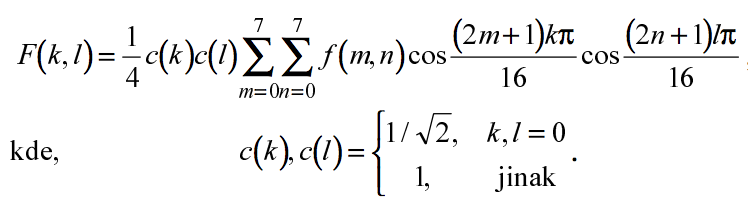
\includegraphics[width=0.8\textwidth]{assets/7_dct1}
		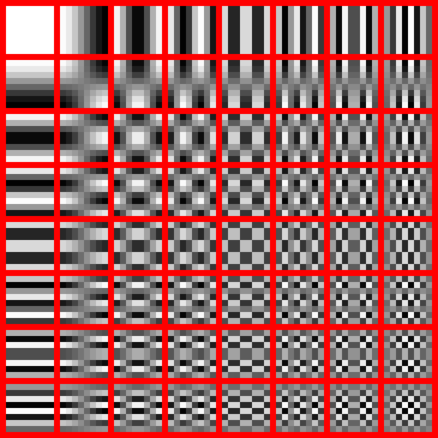
\includegraphics[width=0.3\textwidth]{assets/7_dct2}
		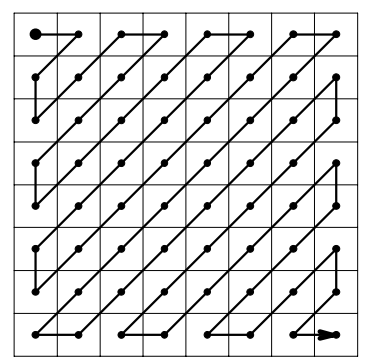
\includegraphics[width=0.35\textwidth]{assets/7_jpeg_zigzag}
	\end{figure}
	\item \textbf{Kvantizace} -- jednotlivé bloky jsou \textbf{vyděleny kvantizační maticí a zaokrouhleny}. Koeficienty matice definují \textbf{míru komprese} (čím větší hodnoty tím větší komprese a horší obraz). Většinou po aplikaci kvantizace v každém bloku zůstane pouze několik hodnot \textbf{vlevo nahoře} to vyplývá z toho co jsme zmínil výše $\rightarrow$ více se redukují vysoké frekvence, které si můžeme dovolit vynechat. Výsledek před a po kvantizaci je vidět obrázku níže.
	\begin{figure}[H]
		\centering
		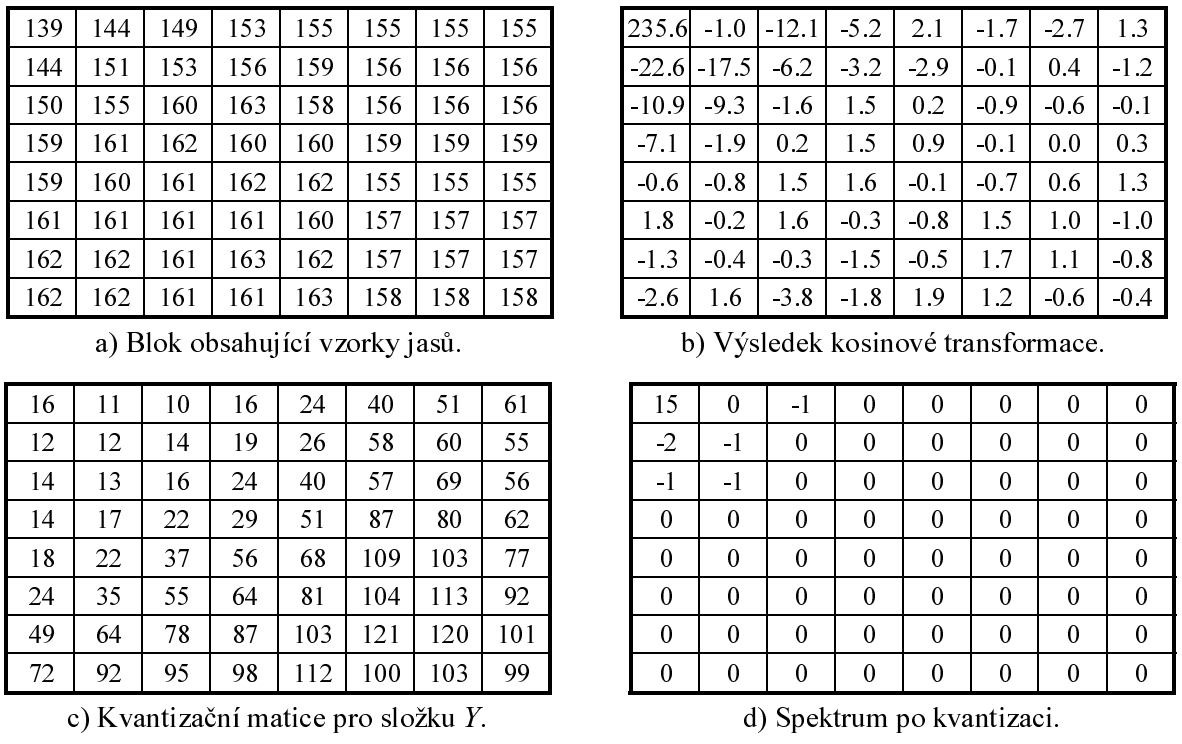
\includegraphics[width=0.8\textwidth]{assets/7_kvantizace}
	\end{figure}
	\item \textbf{Zig-zag intermediální sekvence} -- obraz po kvantizaci se projde \textbf{zig-zagem} a z daných čísel se vytvoří intermediální sekvence (\textbf{dvojice} ve tvaru \textbf{Symbol-1}, \textbf{Symbol-2}) pomocí \textbf{Run-Length encoding}. RLE kóduje pouze AC složky (1 - 64), DC složka (px na souřadnicích [0, 0] každého bloku) se kóduje \textbf{diferenciálně} vzhledem k DC složce v předchozím bloku. Intermediální sekvence vypadá následovně:
	\begin{itemize}
		\item \textbf{Symbol-2} -- (AMPLITUDE) značí hodnotu na daném pixelu po kvantizaci.
		\item \textbf{Symbol-1} -- (RUNLENGTH, SIZE), kde RUNLENGTH značí počet nul, které danému prvku předchází v zig-zag sekvenci (pokud je počet větší než 15, zapíše se 15) a SIZE je počet bitů nutných k reprezentaci AMPLITUDE. \textbf{Speciální hodnota} (0, 0) říká, že předchozí nenulová hodnota byla poslední.
		\item \textbf{Kódování} -- \textbf{DC} složky se kódují odlišně (SIZE, AMPLITUDE), \textbf{AC} složky ((AMPLITUDE), (RUNLENGTH, SIZE).
	\end{itemize}
	Intermediální sekvence se poté zakóduje \textbf{Huffmanovým kódem}, kde se kódují pouze kombinace (RUNLENGTH, SIZE) u AC a (SIZE) u DC podle předem daných tabulek. AMPLITUDE se zapisuje pomocí \textbf{jednotkového doplňku} (způsob reprezentace záporných čísel).
	\begin{figure}[H]
		\centering
		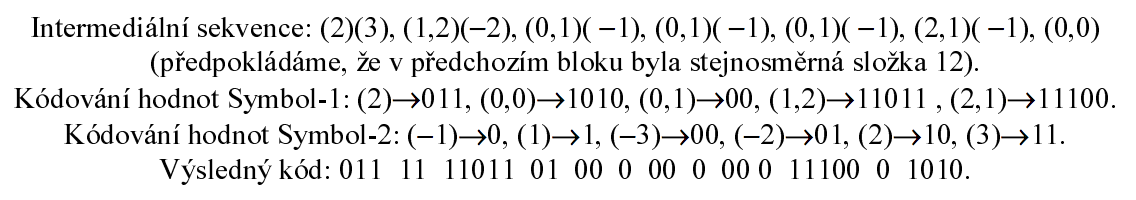
\includegraphics[width=\textwidth]{assets/7_intermediate}
	\end{figure}
\end{enumerate}

\subsection{MPEG}
MPEG je zkratkou pro Moving Picture Expert Group. Cílem práce této skupiny bylo standardizovat metody komprese videosignálu. Existuje několik standardů MPEG-(1, 2, 4, 7). 

\begin{figure}[H]
	\centering
	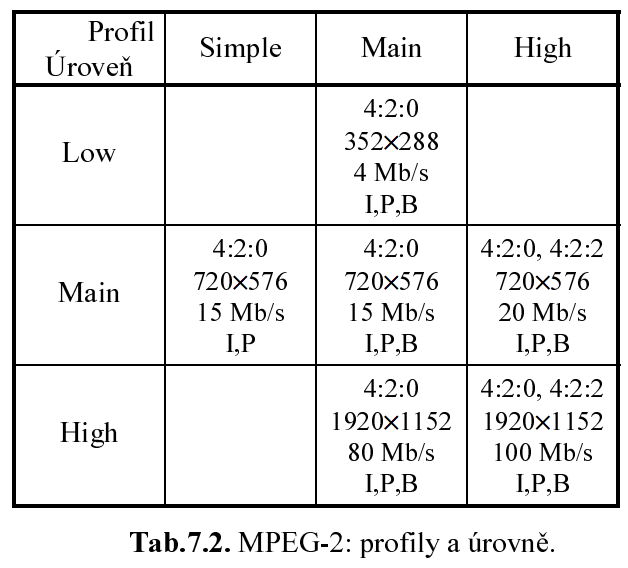
\includegraphics[width=0.5\textwidth]{assets/7_mpeg}
\end{figure}

\begin{itemize}
\item \textbf{MPEG-1} -- první standard, dokončen v roce 1991. Navržen zejména pro práci s obrazy $352\times288$ pixelů, 25FPS (odvozeno od televizní normy PAL) nebo $352\times240$, 30FPS (odvozeno od NTSC) při datovém toku \textbf{1.5 MBit/s} (optimální tok, mohl být i vyšší).
\item \textbf{MPEG-2} -- dokončen v roce 1994, mnohem velkorysejší implementace, snaží se být co \textbf{nejuniverzálnější}. Zavádí několik \textbf{profilů} (podmnožina z nejširší možné syntaxe) a \textbf{úrovní} (definuje parametry v rámci daného profilu).
\item \textbf{MPEG-3} -- práce na tomto standardu byly zastaveny (měl sloužit pro HDTV) později byl sloučen do MPEG-2.
\item \textbf{MPEG-4} -- metodou komprese se značně liší oproti MPEG-1,2, je určen pro \textbf{extrémně nízké datové toky}.
\item \textbf{MPEG-7} -- neříká nic o kódování, jedná se o standard pro popis dat (\textbf{metadata}) s multimediálním obsahem.
\end{itemize}

\subsubsection{Komprese MPEG}
Standard MPEG, rozlišuje \textbf{tři typy rámců (I, B, P)},  ve své podstatě pro kódování využívá stejných principů jako JPEG (\textbf{rámec I} se kóduje nezávisle). Oproti JPEG však využívá i \textbf{časové koherence}. Tedy k dosažení maximální komprese se předpokládá, že po sobě jdoucí rámce jsou s největší pravděpodobností dosti podobné. Počítá se ovšem s tím, že části obrazů se mohou přemístit, k tomu se využívá vložených rámců P a B, které se kódují \textbf{závisle} vzhledem k ostatním.
\begin{itemize}
\item \textbf{I} -- jsou kódovány každý \textbf{zvlášť}, bez vazby na rámce předcházející či následující. Pricip kódování (komprese) je stejný jako u standardu \textbf{JPEG} (i když v detailech existují některé \textbf{odlišnosti}: jiná kvantovací tabulka, jiná struktura intermediální sekvence a jiný způsob \textbf{zig-zagu} (podle MPEG-2)). \textbf{Kvantizační tabulka} může být pro každý makroblok jiná -- změnou měřítka lze \textbf{řídit tok dat} (některé aplikace mohou vyžadovat konstantní tok dat).
\item \textbf{P (Predicted)} -- tento rámec je kódován \textbf{vzhledem k jedinému předcházejícímu rámci typu I nebo P}. 
\item \textbf{B (Interpolated bi-directionally)} -- tyto rámce jsou kódovány vzhledem k nejbližšímu \textbf{předchozímu} a \textbf{nejbližšímu} budoucímu rámci typu \textbf{I} nebo \textbf{P}. Jejich použití je nepovinné ale z hlediska dosahovaných kompresních poměrů výhodné. \textbf{Komplikace} z použití rámců B spočívá v uchovávání v paměti dva kotevní obrazy. Dále je nevyhnutelné jisté časové zpoždění, protože nejprve musí být k dispozici obraz \textbf{novější} a teprve potom může být kódován obraz starší.
\begin{figure}[H]
	\centering
	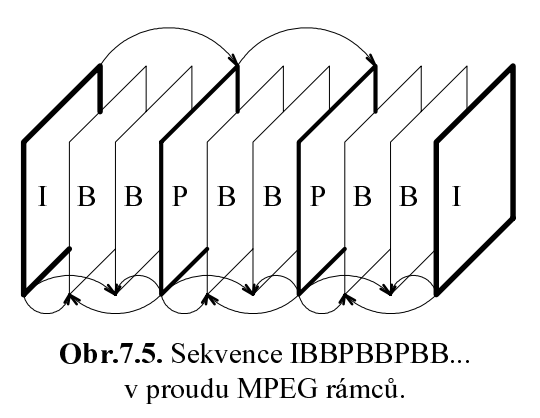
\includegraphics[width=0.48\textwidth]{assets/7_mpeg_komprese}
	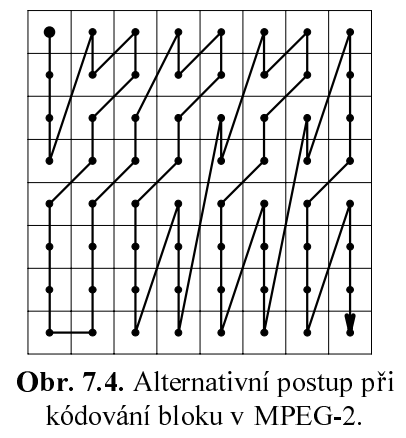
\includegraphics[width=0.35\textwidth]{assets/7_mpeg_zigzag}
\end{figure}
\end{itemize}

Velmi často používané řazení rámců je IBBPBBPBBI. Kódování rámců P a B taky probíhá po \textbf{makroblocích}. Pro každý makroblok v cílovém (tj. právě kódovaném rámci) jsou sestaveny \textbf{vektory pohybu} (pro každý makroblok v P \textbf{jeden} vektor, v B jsou vektory \textbf{dva}) vzhledem k referenčním rámcům.

\textbf{Vektor pohybu} je definován takto: jestliže o uvedený vektor posuneme kódovaný makroblok a porovnáme s odpovídající částí referenčního obrazu, pak je dosaženo dobré shody. Vektory posunutí se stávají \textbf{součástí komprimované} sekvence. Po nalezení vektoru jsou \textbf{kódovány diference} -- podobně jako u JPEGu mezi odpovídajícími makrobloky bude v dvou rámcích \textbf{malý rozdíl} a výsledné data po kvantizaci vyžadují tak \textbf{malé sekvence} (komprese).
\begin{itemize}
\item Bloky \textbf{P} se kódují $T-R$, kde T je makroblok v cílovém rámci,
\item bloky \textbf{B} se kódují $T - 0.5 (R_1 + R_2)$, kde $R_1$ a $R_2$ jsou makrobloky v cílových rámcích.
\end{itemize}

\begin{figure}[H]
	\centering
	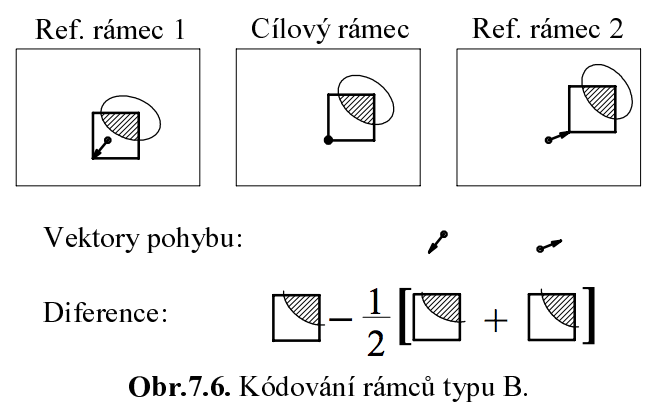
\includegraphics[width=0.48\textwidth]{assets/7_mpeg_kodovani_B}
\end{figure}

\subsubsection{Stanovení pohybového vektoru}
Stanovení pohybového vektoru MPEG norma nepředepisuje, jedná se však o jeden z \textbf{nejobtížnějších problémů}. Většinou se využívá pouze \textbf{jasové} (Y) složky, existuje několik metod:

\begin{enumerate}
\item \textbf{Porovnání makrobloků} -- v referenčním rámci se nalezne makroblok, který nejvíce odpovídá zpracovávanému makrobloku. Pro určení shody lze použít např. SSD. \textbf{Účinné}, avšak velmi \textbf{časově náročné}.
\item \textbf{Logaritmické vyhledávání} -- vylepšení předchozí metody, má logaritmickou časovou složitost. V prvním kroku algoritmus testuje 9 dvojic. V každém dalším kroku se testuje vždy po 8 dvojicích rozmístěných kolem předchozího bodu, který měl největší shodu. Rychlejší, ale nemusí být tak přesné jak předchozí metoda.
\item \textbf{Rekurzivní dělení} -- rekurzivně dělíme obraz na menší a menší. Poté nalezneme prvotní odhad v nejmenším obraze a se zvyšující se velikostí (návrat z rekurze) pozici vektoru jen upřesňujeme. Rychlé a spolehlivé.
\end{enumerate}

\begin{figure}[H]
	\centering
	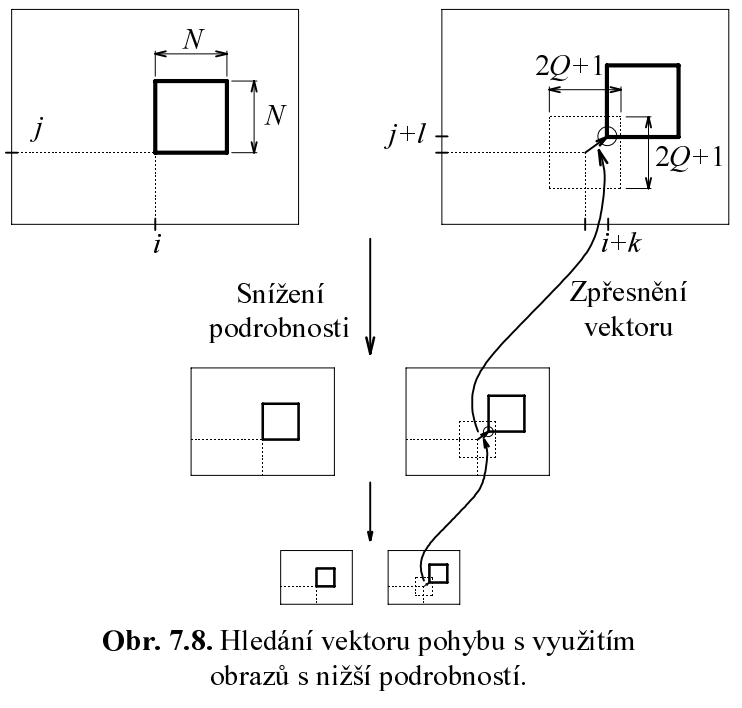
\includegraphics[width=0.48\textwidth]{assets/7_mpeg_rekurze}
	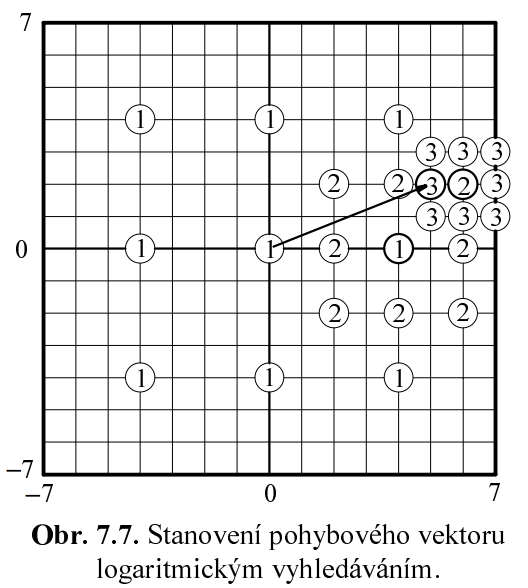
\includegraphics[width=0.48\textwidth]{assets/7_mpeg_log}
\end{figure}

Kódování složek vektorů se provádí \textbf{inkrementálně vzhledem k předchozí hodnotě}. Zároveň může nastat situace kdy se vektor nepodaří nalézt, v tom případě je možné kódovat dané makrobloky nezávisle na ostatních (stejně jako I).

\begin{figure}[H]
	\centering
	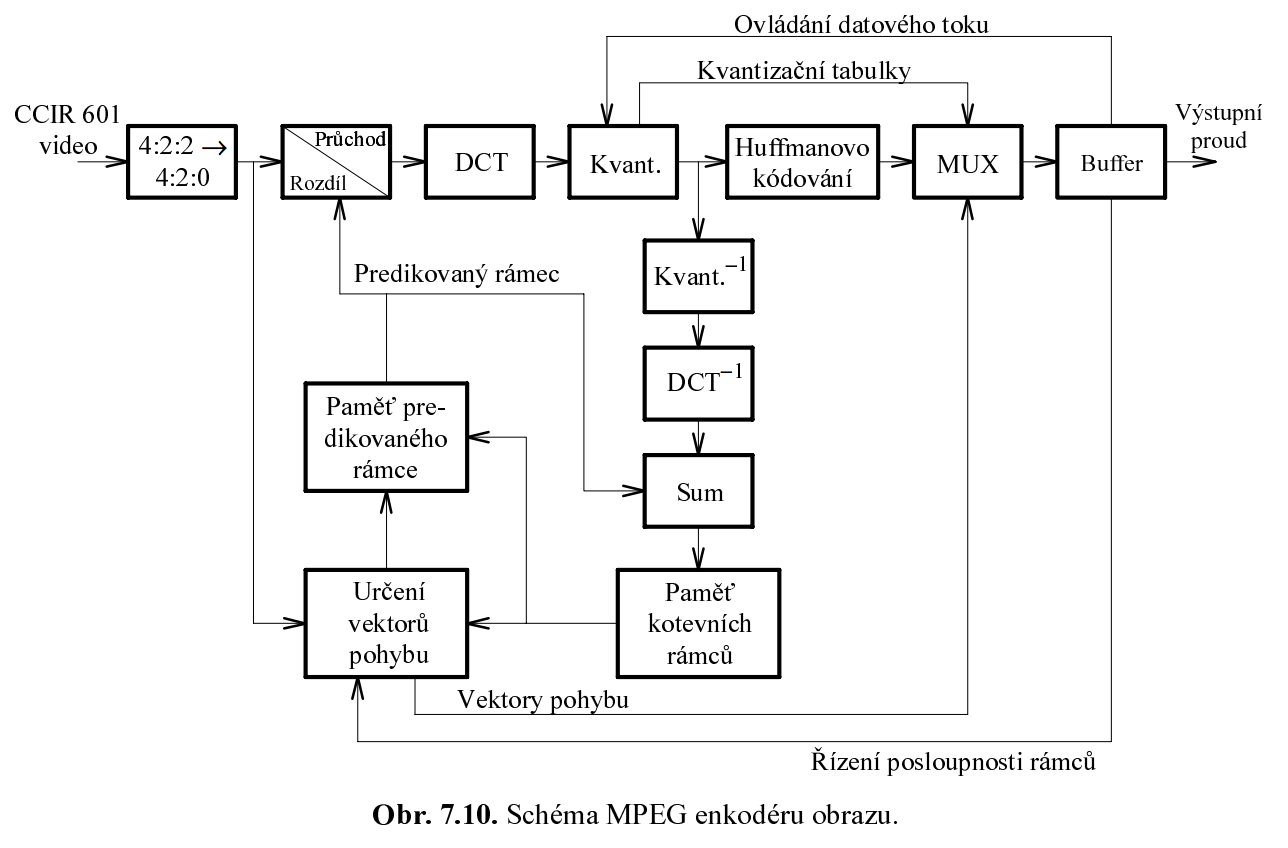
\includegraphics[width=\textwidth]{assets/7_mpeg_schema}
\end{figure}

\subsection{Principy úprav obrazu v prostorové a frekvenční doméně}

% Furier a úpravy + konvoluce



